%=========================================================================
% (c) 2011, 2012 Josef Lusticky

\chapter{Network Time Protocol}
Network Time Protocol provides mechanism for synchronising systems' clocks over the variable-latency data network.
NTP was introduced and is still developed by
David Mills at University of Delaware in Newark, United States of America~\cite{ntp-history}.
NTP is arguably the longest running, continuously operating,
ubiquitously available protocol in the Internet~\cite{ntp-overview}.
Despite being one of the oldest surviving protocols on the Internet, it is not old-fashioned at all.
NTP version 4 described in RFC~5905~\cite{rfc5905} is an update to older NTPv3 to accommodate NTP to IPv6.
Version 4 also includes improvements in
mitigation and clock discipline algorithms that extend
potential accuracy to the tens of microseconds with modern
workstations and fast LANs~\cite{rfc5905}.
NTPv4 corrects some
errors in NTPv3 design and includes optional extension mechanism
that can be used for adding more capabilities to NTP, e.g. the
Autokey security protocol described in RFC~5906
for authenticating servers to clients.

Simple Network Time Protocol is simplified NTP implementation lacking complex
synchronisation algorithms used by NTP~\cite{rfc5905}.
SNTP is also described in RFC 5905.
The packets of SNTP have the same structure and content as packets of NTP~\cite{rfc5905}.
From observing the network communication, one can not tell, whether the client
is full blown NTP implementation or just SNTP.
SNTP is a simplified sub-set of algorithms used by the NTP protocol
making the client implementation not only easier, but also suitable for
resource constraint systems such as embedded systems.
Since NTP and SNTP servers and clients are
completely interoperable and can be intermixed in NTP subnets~\cite{rfc5905},
this thesis refers to SNTP client for Contiki OS as NTP client.


%=========================================================================
% (c) 2011, 2012 Josef Lusticky

\section{Topology and hierarchy}\label{sec:ntp-topology}
NTP uses two different communication modes:
one to one, referred as unicast mode, and one to many, referred as broadcast mode~\cite{rfc5905}.
In unicast communication mode, NTP client sends request and NTP server sends response.
In broadcast communication mode, the client sends no request
and waits for a broadcast message from one or more servers~\cite{rfc5905}.

NTP servers are rated with stratum (plural form strata) number which represents their position
in an NTP hierarchy and their possible accuracy~\cite{rfc5905}.
Primary (stratum 1) servers synchronise to the reference clock directly traceable to UTC via
radio, satellite or modem.
The stratum 2 servers synchronise to stratum 1
servers via hierarchical subnet.
The stratum 3 servers synchronise to stratum 2 servers, and so on.
The maximum stratum is 15, number 16 means unsynchronised server
and higher numbers (up to 255) are reserved~\cite{rfc5905}.
Synchronisation between servers in the same stratum level is also possible.
Figure~\ref{fig:ntp-hierarchy} shows a brief hierarchy of NTP.
\begin{figure}
  \centering
  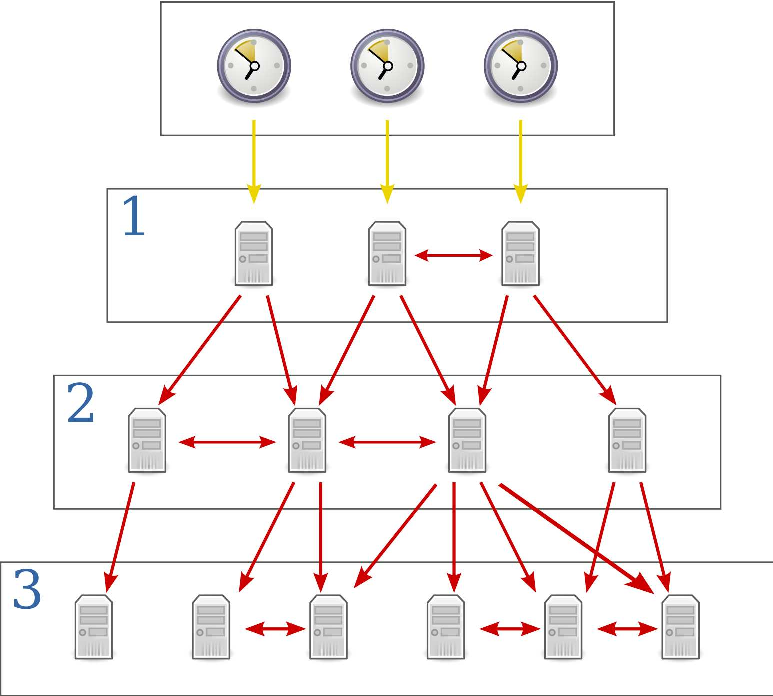
\includegraphics[width=9cm,keepaspectratio]{fig/Network_Time_Protocol_servers_and_clients.pdf}
  \caption{Topology and hierarchy of NTP by B. Esham}
  \label{fig:ntp-hierarchy}
  \bigskip
\end{figure}


%=========================================================================
% (c) 2011, 2012 Josef Lusticky <xlusti00@stud.fit.vutbr.cz>

\section{Time and timescales}\label{sec:ntp-time}
For expressing the time NTP always uses the Coordinated Universal Time (UTC)~\cite{rfc5905}.
UTC is maintained by the International Bureau of Weights and Measures in Paris, France.
It is the time scale that forms the basis for coordinated dissemination
of standard frequencies and time signals~\cite{bipm-utc}.
The time specified by UTC is the same for all timezones.
Its calculation is the same as with Greenwich Mean Time (GMT),
however the daylight savings are not accounted.

The UTC scale is adjusted by the insertion of leap seconds to ensure approximate
agreement with the time derived from the rotation of the Earth~\cite{bipm-utc}.
The atomic clocks, on which UTC is based, are so precise that
they do not match the rotation of the Earth,
which periodically speeds up and slows down due to the action
of tides and changes within the Earth's core~\cite{cnn-earth}.
The goal of a leap second is to catch up UTC with these changes.
The leap second is inserted or deleted on the advice of
International Earth Rotation and Reference Systems Service~\cite{bipm-utc}.
NTP is well designed for leap second occurrence -
there is Leap Indicator field
in the structure of NTP packet and there are also fields intended for
information about leap second in structures that NTP algorithm uses~\cite{rfc5905}.
The formal definition of UTC does not permit double leap seconds~\cite{posix}.

In computer the system time is represented by system clock maintained by
hardware and operating system.
The goal of the NTP algorithms is to minimize
both the time difference and frequency difference between UTC and the system clock.
When these differences have been reduced below nominal
tolerances, the system clock is said to be synchronised to UTC~\cite{rfc5905}.
It has never been a goal of NTP to take care of local time,
it is up to operating system to provide user the correct local time~\cite{ntp-overview}.

The NTP and POSIX timescales are based on the UTC timescale,
but not always coincident with it~\cite{ntp-leap}.
Both timescales reckon in seconds since the prime epoch,
but the origin of the NTP timescale, the NTP prime epoch, is 00:00:00 UTC on 1 January 1900,
while the prime epoch of the POSIX timescale is 00:00:00 UTC on 1st January 1970~\cite{ntp-leap}.
%! VYHODIT?
So upon the first tick of POSIX clock on 1st January 1970 the NTP clock read 2~208~988~800,
representing the number of seconds since the NTP prime epoch.
Some of interesting dates with their respective NTP time values
can be found in appendix~\ref{app:dates}.


%=========================================================================
% (c) 2011, 2012 Josef Lusticky <xlusti00@stud.fit.vutbr.cz>

\section{Network and timestamps}\label{sec:ntp-network}
Network specification of NTP defines that
the protocol uses the User Datagram Protocol (UDP) on port number 123~\cite{ianna-ports,rfc5905}.
Reliable message delivery such as TCP can actually make the delivered NTP packet less reliable since retries
would increase the delay value and other errors~\cite{rfc5905}.
This is mostly due to overhead of communication with TCP on transport layer.

NTP manipulates with the time through timestamps - a record of time.
NTP timestamp has two fields. The seconds field expressing the number of seconds
and the fraction field expressing fraction of a second~\cite{rfc5905}.
All NTP time values are represented in twos-complement format, with
bits numbered in big-endian fashion from zero starting at the left, or high-order, position~\cite{rfc5905}. 
There are two formats of timestamp in NTP packet structure:
long 64-bit and short 32-bit as shown on figure~\ref{fig:ntp-timestamps}.
The 64-bit long timestamp used by NTP consists of a 32-bit unsigned seconds
field spanning $2^{32}$ seconds (aprox. 136 years from 1900 to 2036) and a 32-bit fraction field resolving
$2^{-32}$ seconds (aprox. 232 picoseconds)~\cite{rfc5905}.
The short 32-bit timestamp includes a 16-bit unsigned seconds field
and 16-bit fraction field.

There is one more NTP time format - 128-bit date format.
This format is however not transmitted over the network
and since this 128-bit date format is used where sufficient storage and word
size are available~\cite{rfc5905},
there is practically no need of knowing about this format for embedded systems.
But strictly speaking an NTP timestamp is a truncated NTP date format~\cite{rfc5905}.

\begin{figure}
	\centering
	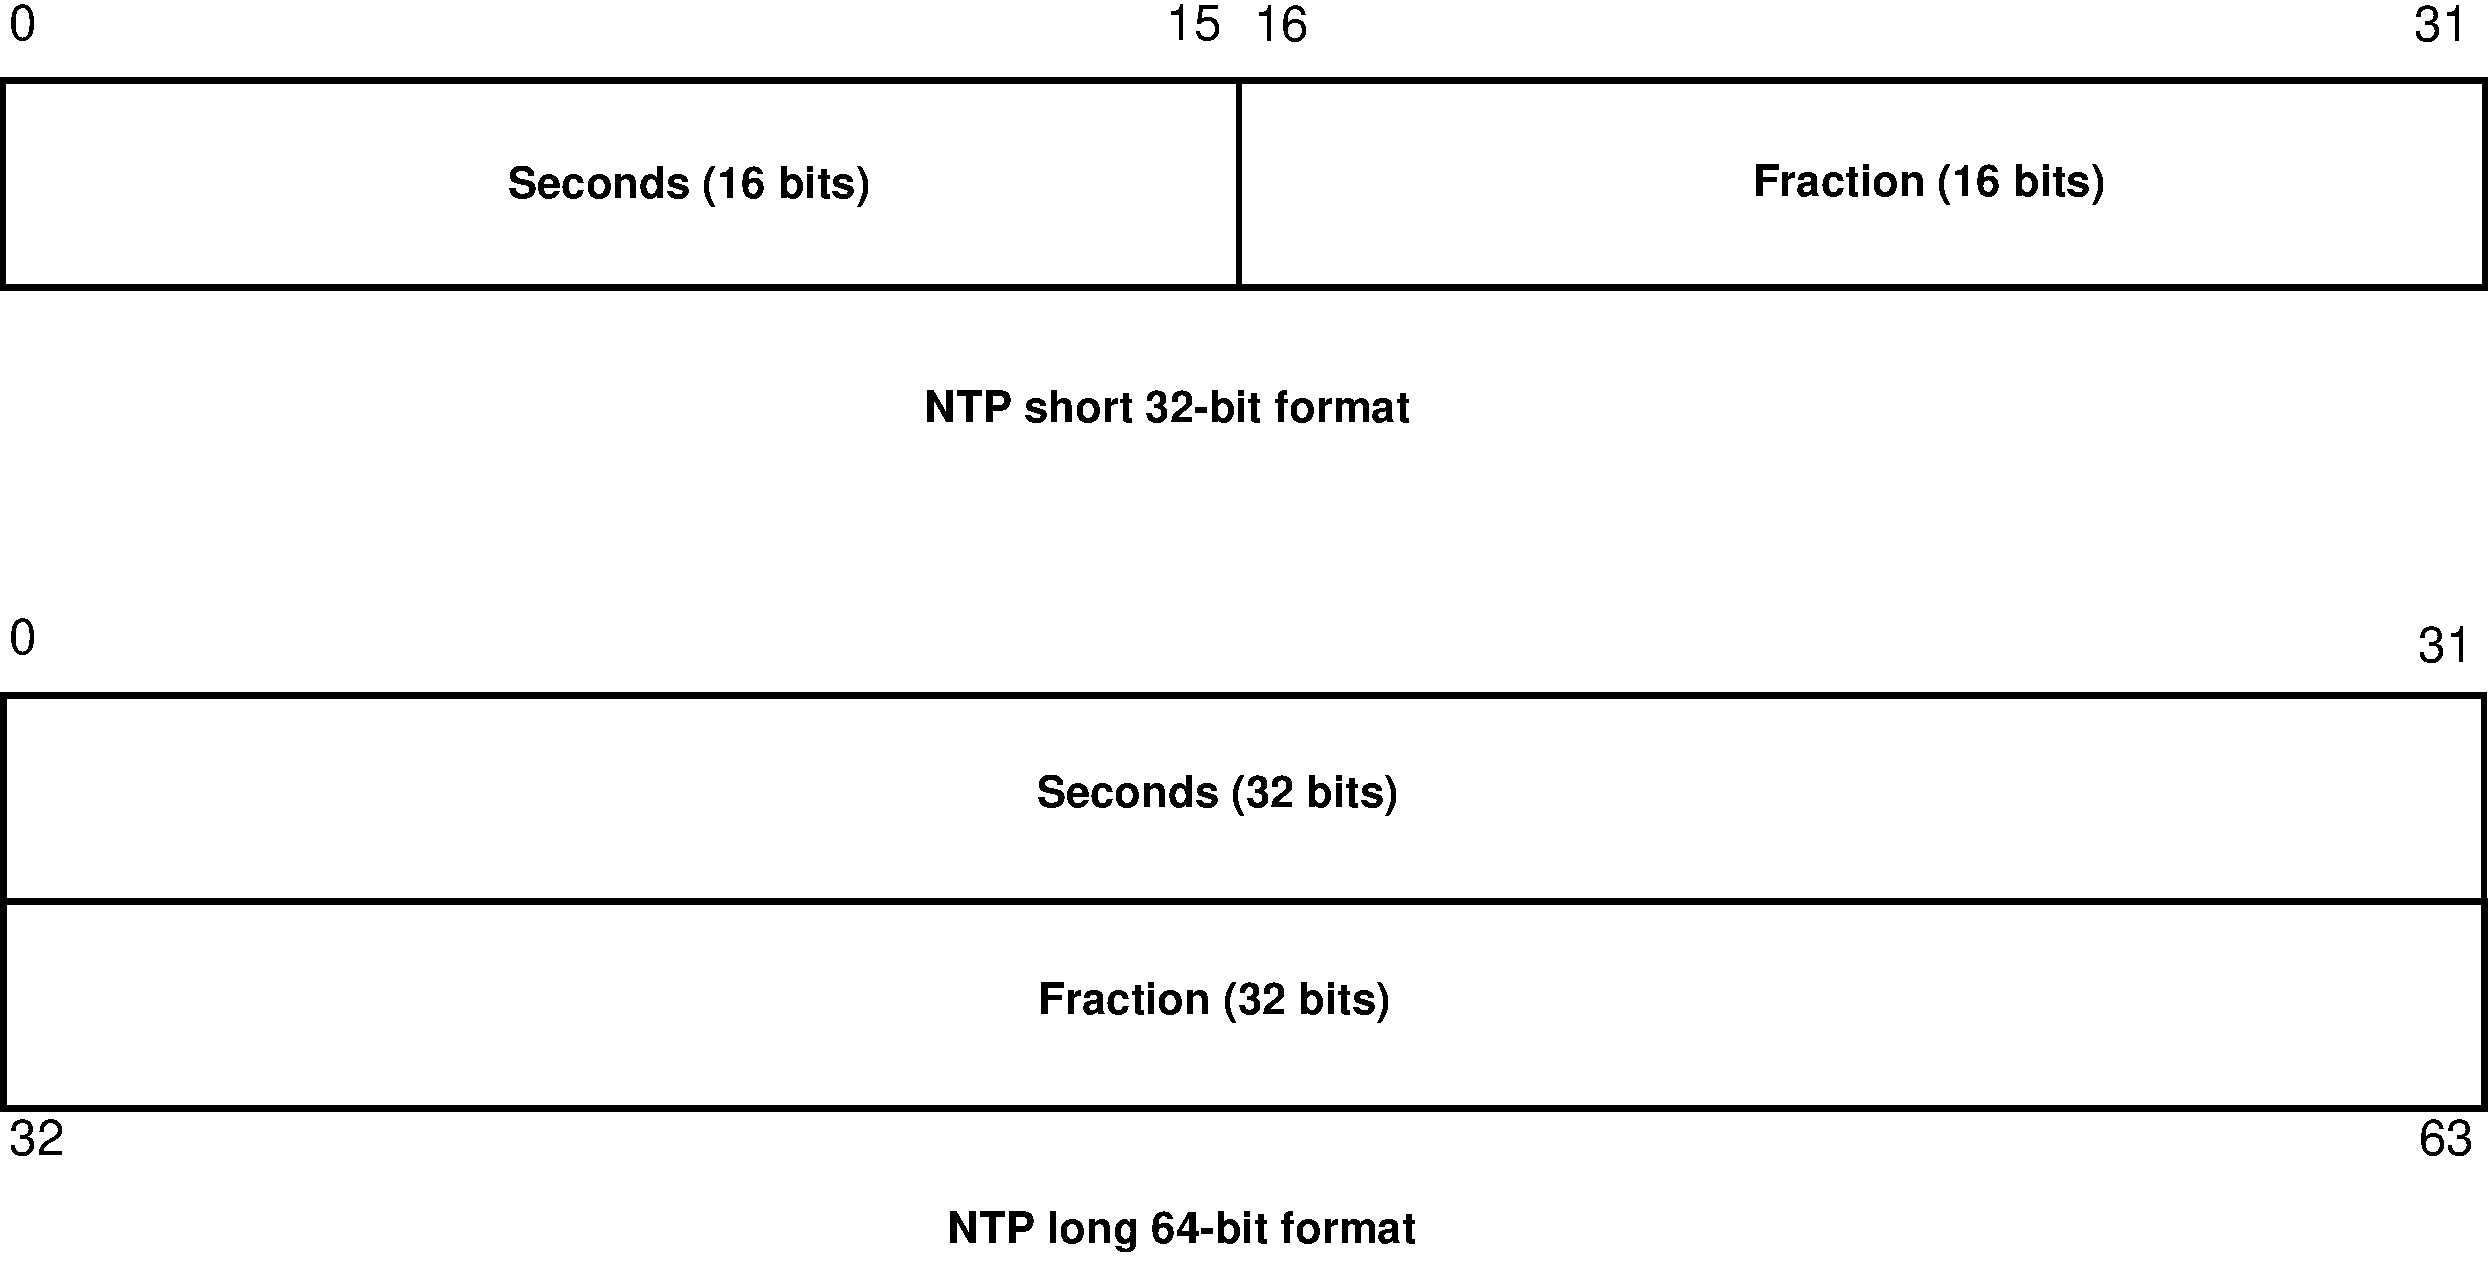
\includegraphics[width=13cm,keepaspectratio]{fig/ntp-timestamps.pdf}
	\caption{Time formats used in NTP packet}
	\label{fig:ntp-timestamps}
	\bigskip
\end{figure}

% TODO - packet

\begin{figure}
	\centering
	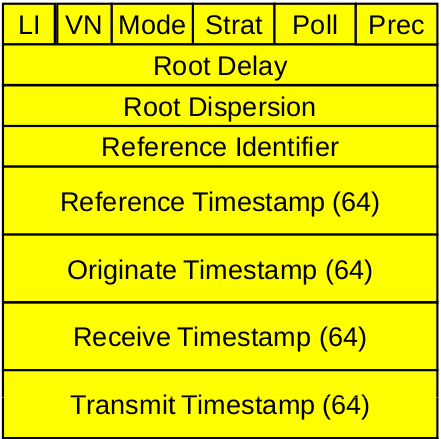
\includegraphics[width=6cm,keepaspectratio]{fig/ntp-packet.png}
	\caption{Basic NTP packet structure}
	\label{fig:ntp-packet}
	\bigskip
\end{figure}


Because the short 32-bit format is used for Root dispersion and Root Delay fields,
they do not need so big scope and precision.
Root dispersion express accumulated total dispersion from primary server
and Root Delay express accumulated roundtrip delay via primary server~\cite{ntp-arch}.

%TODO

Because of network latency the timestamp recieved will never be exactly corresponding to
the current time.
One of the main goals of NTP is to deal with the network latency~\cite{ntp-overview}.



%=========================================================================
% (c) 2011, 2012 Josef Lusticky

\section{Algorithms}\label{sec:ntp-algorithms}
Because of network latency the received Transmit Timestamp will never be exactly
corresponding to the current time.
One of the main goals of NTP is to deal with the network latency~\cite{ntp-overview}.

As described in section~\ref{sec:ntp-network},
there are the following 64-bit long timestamps in NTP packet: Origin, Receive and Transmit Timestamp.
Upon NTP packet arrival, the client determines another timestamp called
Destination Timestamp~\cite{rfc5905}.
This timestamp is represented as T4 on figure~\ref{fig:ntp-client-server}
and is not part of NTP packet structure.

Using these four timestamps, NTP client using unicast communication mode can compute
the local clock offset which is given by $\theta = \frac{1}{2}[(t_2 - t_1) + (t_3 - t_4)]$,
where $t_1$ is the time of the request packet transmission (Origin Timestamp),
$t_2$ is the time of the request packet reception (Receive Timestamp),
$t_3$ is the time of the response packet transmission (Transmit Timestamp) and
$t_4$ is the time of the response packet reception (Destination Timestamp)~\cite{ntp-algor,rfc5905}.
The implicit assumption in the above is that one-way delay is
statistically half of round-trip delay~\cite{rfc5905},
which is given by $\delta = (t_4 - t_1) - (t_3 - t_2)$.

In broadcast communication mode, Origin and Receive Timestamps are not accounted.
The client computes its local clock offset which is given by $\theta = t_3 - t_4$.
The implicit assumption in the above is that one-way delay from server to client is zero.
Since this is never the case, it is useful to provide an
initial volley where the client exchanges several packets with the server in
order to calibrate the propagation delay~\cite{rfc5905}.

When computing the result from more servers, the intersection algorithm is used
for selecting the possible most exact timestamp received from various servers~\cite{ntp-improved-algor,rfc5905}.
Intersection algorithm is derived from Murzollo algorithm but the basic
computation remains the same~\cite{ntp-history}.
First of all a selection of bad and good servers must be made.
Bad servers are called Falsetickers and good are called Truechimers~\cite{rfc5905}.
The division to these sets is based on their response.
As one can assume for a sensible result there must be more Truechimers than Falsetickers~\cite{rfc5905}.

After selecting a set of reliable servers, NTP clock algorithms compute resulting exact timestamp.
The resulting exact timestamp does not have to be the same
as one of those provided by the servers.
NTP clock algorithms calculate using clock accuracy estimates
determined from Root Dispersion, Root Delay and Precision fields of server's response.
These estimates are converted to intervals.
Figure~\ref{fig:ntp-intersection} shows the computation for the following example:
If we have the estimates $10 \pm 2$, $12 \pm 1$ and $11 \pm 1$
then these intervals are $<8; 12>$, $<11; 13>$ and $<10; 12>$ which
intersect to form $<11; 12>$ or $11.5 \pm 0.5$ as consistent with all three values.
The arithmetic mean is used as the result value.
When querying servers again, the algorithm repeats but the new result computation
also depends on the previous result~\cite{rfc5905,ntp-history}.
This eliminates possible jitter which can be caused by repeatedly querying the servers
and getting slightly different answers from them.

\begin{figure}
	\centering
	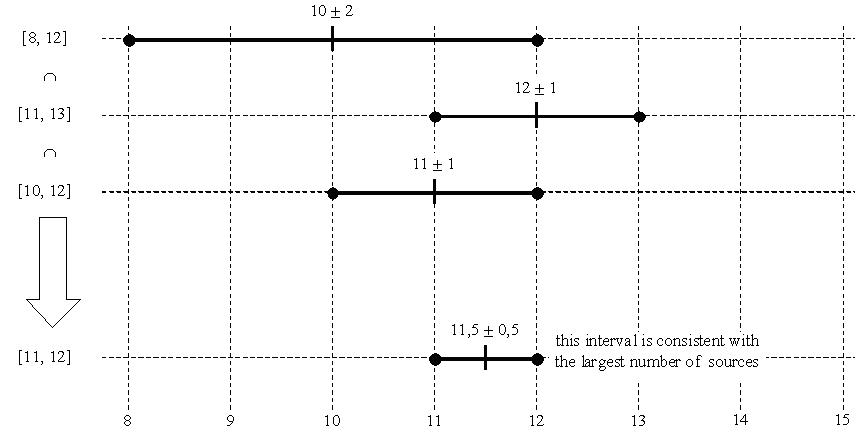
\includegraphics[width=13cm,keepaspectratio]{fig/Marzullo_example-1.jpg}
	\caption{Intersection algorithm by D. Exb}
	\label{fig:ntp-intersection}
	\bigskip
\end{figure}

%Since the clients complying with a subset of NTP, called
%the Simple Network Time Protocol (SNTPv4) [RFC4330], do not need to
%implement the mitigation algorithms ... ~\cite{rfc5905}.

